\documentclass[12pt]{article}
\usepackage{pdfpages}
\usepackage{tabularx}
\usepackage{graphicx}
\usepackage{hyperref}
\usepackage{xcolor}
\hypersetup{
    colorlinks,
    linkcolor={red!50!black},
    citecolor={blue!50!black},
    urlcolor={blue!80!black}
}
\usepackage{bm}
\usepackage{natbib}
\usepackage{longtable}
\LTcapwidth=0.87\textwidth



\newcommand{\sol}{\ensuremath{\odot}}
\newcommand{\RB}{Rayleigh-B\'{e}nard }

\def\changemargin#1#2{\list{}{\rightmargin#2\leftmargin#1}\item[]}
\let\endchangemargin=\endlist

\parskip=0.021in
\parindent=0.17in
\textwidth=6.5in
\textheight=8.99in
\topmargin=-0.53in
\oddsidemargin=0.0in
\evensidemargin=0.0in

\usepackage{fancyhdr}
\pagestyle{fancy}
\fancyhf{} % sets both header and footer to nothing
\renewcommand{\headrulewidth}{0pt}
\cfoot{\footnotesize{\thepage}}
\rfoot{\footnotesize{Evan H. Anders, NASA NESSF 2018}}



\begin{document}

\begin{center}

\vspace*{0.07in}
Student: \, Evan H. Anders\hspace{0.6cm}

Advisor: \, Benjamin P. Brown

\vspace*{0.15in}
University of Colorado at Boulder, Laboratory for Atmospheric and Space Physics (LASP)

\vspace*{0.15in}
NASA Earth and Space Science Fellowship (NESSF) 2018 \\
Application

\vspace*{0.39in}
{\em Towards a more complete understanding of Stratified, Compressible Convection}

\vspace*{0.44in}
{\bf TABLE OF CONTENTS}
\end{center}

\vspace*{0.33in}
\noindent
1.$\,$ Personal Statement
\dotfill \hyperlink{page.2}{2}

\vspace*{0.06in}
\noindent
2.$\,$ Project Description
\dotfill \hyperlink{page.3}{3}

\vspace*{0.06in}
\noindent\hspace*{0.25in}
2.1.$\,$ Background and Motivation
\dotfill \hyperlink{page.3}{3}

\vspace*{0.06in}
\noindent\hspace*{0.25in}
2.2.$\,$ Proposed Project
\dotfill \hyperlink{page.3}{3}

\vspace*{0.06in}
\noindent\hspace*{0.50in}
2.2.1.$\,$ Internally heated convection
\dotfill \hyperlink{page.3}{3}

\vspace*{0.06in}
\noindent\hspace*{0.50in}
2.2.2.$\,$ Convection with hydrogen ionization
\dotfill \hyperlink{page.3}{3}

\vspace*{0.06in}
\noindent\hspace*{0.50in}
2.2.3.$\,$ Convection with Kramer's opacity
\dotfill \hyperlink{page.3}{3}

\vspace*{0.06in}
\noindent\hspace*{0.25in}
2.3.$\,$ Numerical Tool and Feasibility
\dotfill \hyperlink{page.3}{3}

\vspace*{0.06in}
\noindent\hspace*{0.25in}
2.4.$\,$ Anticipated Timeline
\dotfill \hyperlink{page.3}{3}

\vspace*{0.06in}
\noindent\hspace*{0.25in}
2.5.$\,$ Relevance to NASA
\dotfill \hyperlink{page.3}{3}

\vspace*{0.06in}
\noindent\hspace*{0.25in}
2.5.$\,$ Summary
\dotfill \hyperlink{page.3}{3}

\vspace*{0.06in}
\noindent
3.$\,$ Schedule
\dotfill \hyperlink{page.8}{8}

\vspace*{0.06in}
\noindent
4.$\,$ Curricula Vitae
\dotfill \hyperlink{page.9}{9}

\vspace*{0.06in}
\noindent\hspace*{0.25in}
4.1.$\,$ Benjamin P. Brown, Faculty Advisor
\dotfill \hyperlink{page.10}{10}

\vspace*{0.06in}
\noindent\hspace*{0.25in}
4.2.$\,$ Evan H. Anders, Student
\dotfill \hyperlink{page.11}{11}

\vspace*{0.06in}
\noindent
5.$\,$ Letter of Recommendation
\dotfill \hyperlink{page.12}{12}

\vspace*{0.06in}
\noindent
6.$\,$ Statement of Originality
\dotfill \hyperlink{page.13}{13}

\vspace*{0.06in}
\noindent
7.$\,$ Transcripts
\dotfill \hyperlink{page.14}{14}

\vspace*{0.06in}
\noindent\hspace*{0.25in}
7.1.$\,$ Undergraduate
\dotfill \hyperlink{page.14}{14}

\vspace*{0.06in}
\noindent\hspace*{0.25in}
7.2.$\,$ Graduate
\dotfill \hyperlink{page.16}{16}

%Personal statement
\newpage
\lfoot{\footnotesize{Personal Statement}}
\includepdf[pages=-, pagecommand={}]{personal_statement/statement_nessf2018_EvanAnders.pdf}

%Proposal
\newpage
\lfoot{\footnotesize{Project Description}}
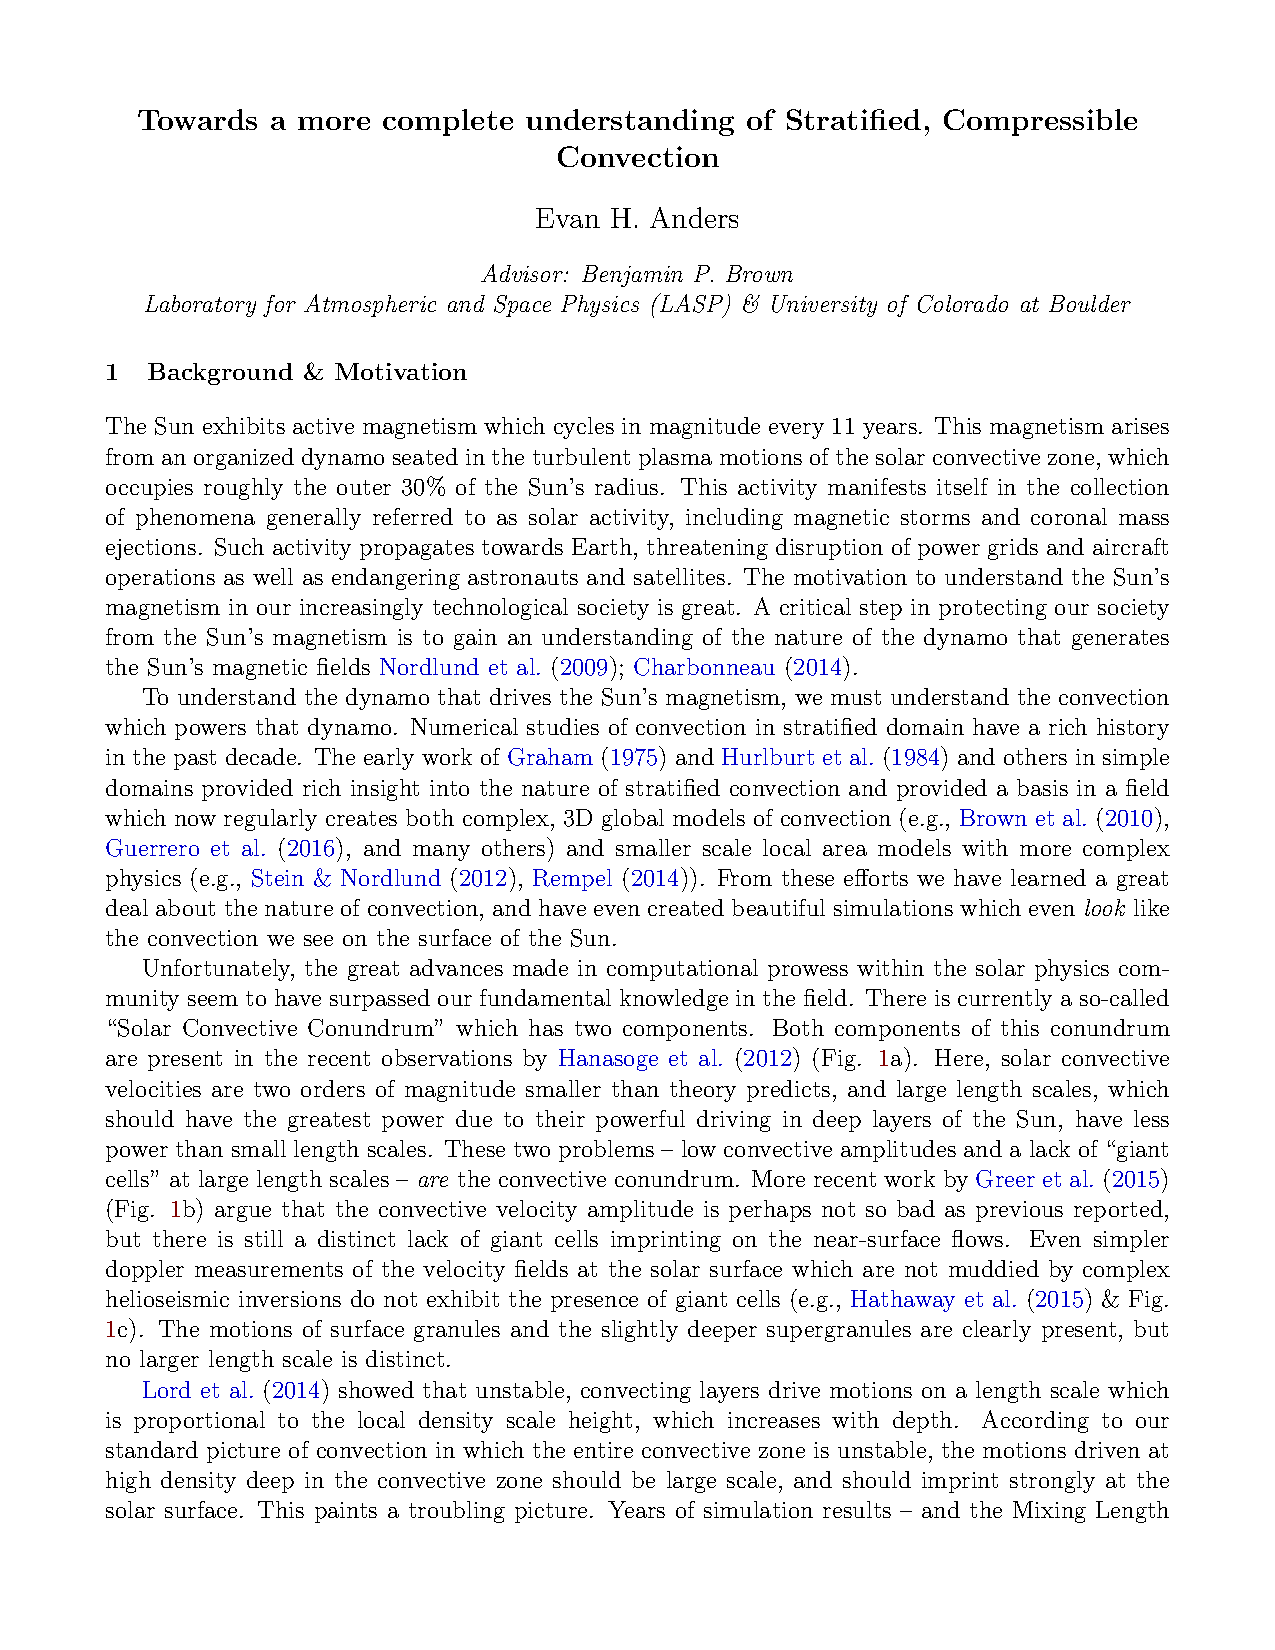
\includepdf[pages=-, pagecommand={}]{research_proposal/proposal_nessf2018_EvanAnders.pdf}

%Schedule
\lfoot{\footnotesize{Schedule}}

%CV -- Ben
\lfoot{\footnotesize{Ben Brown's CV}}

%CV -- Evan
\lfoot{\footnotesize{Evan Anders' CV}}

%Letter of Rec
\lfoot{\footnotesize{Letter of Recommendation}}

%Statement of Originality
\lfoot{\footnotesize{Statement of Originality}}

%Undergrad Transcript
\newpage
\lfoot{\footnotesize{Undergraduate Transcript}}
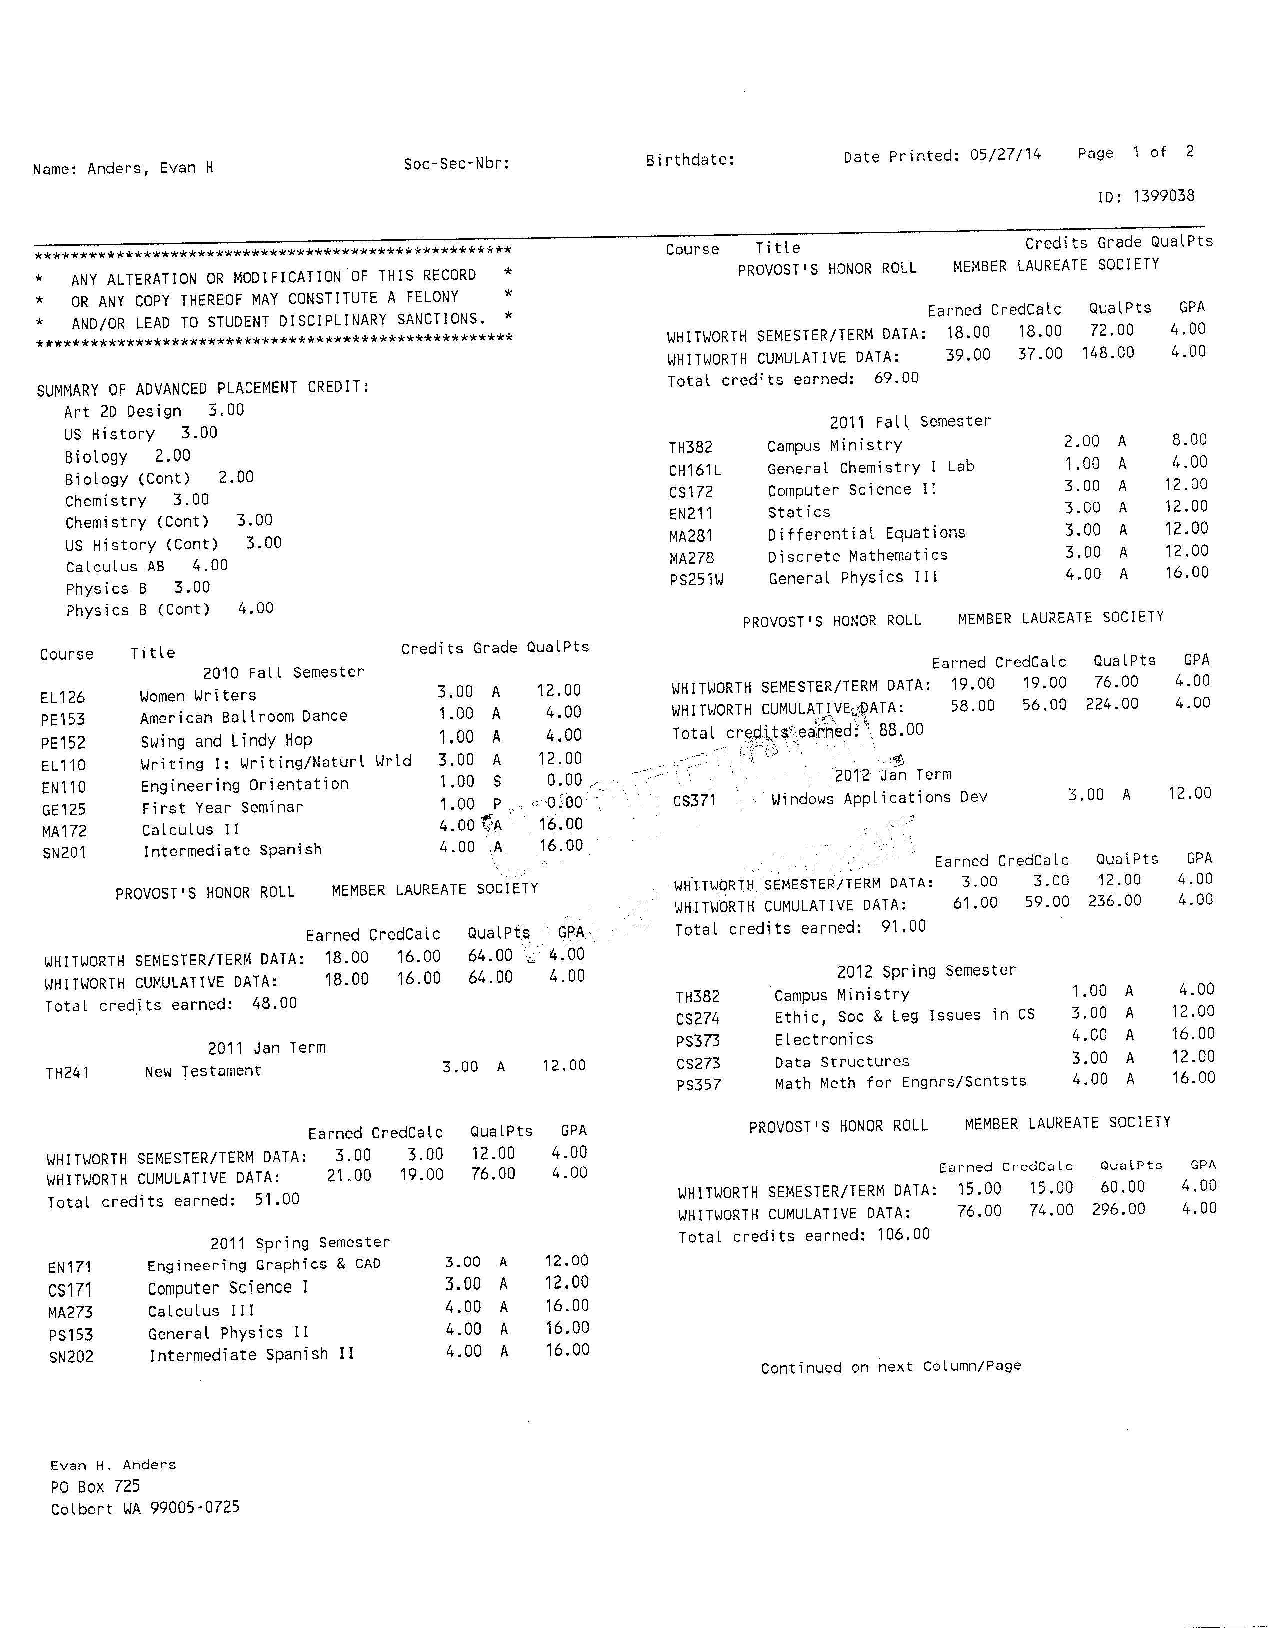
\includepdf[pages=-, pagecommand={}]{transcripts/transcript_whitworth.pdf}

%Grad Transcript
\newpage
\lfoot{\footnotesize{Graduate Transcript}}
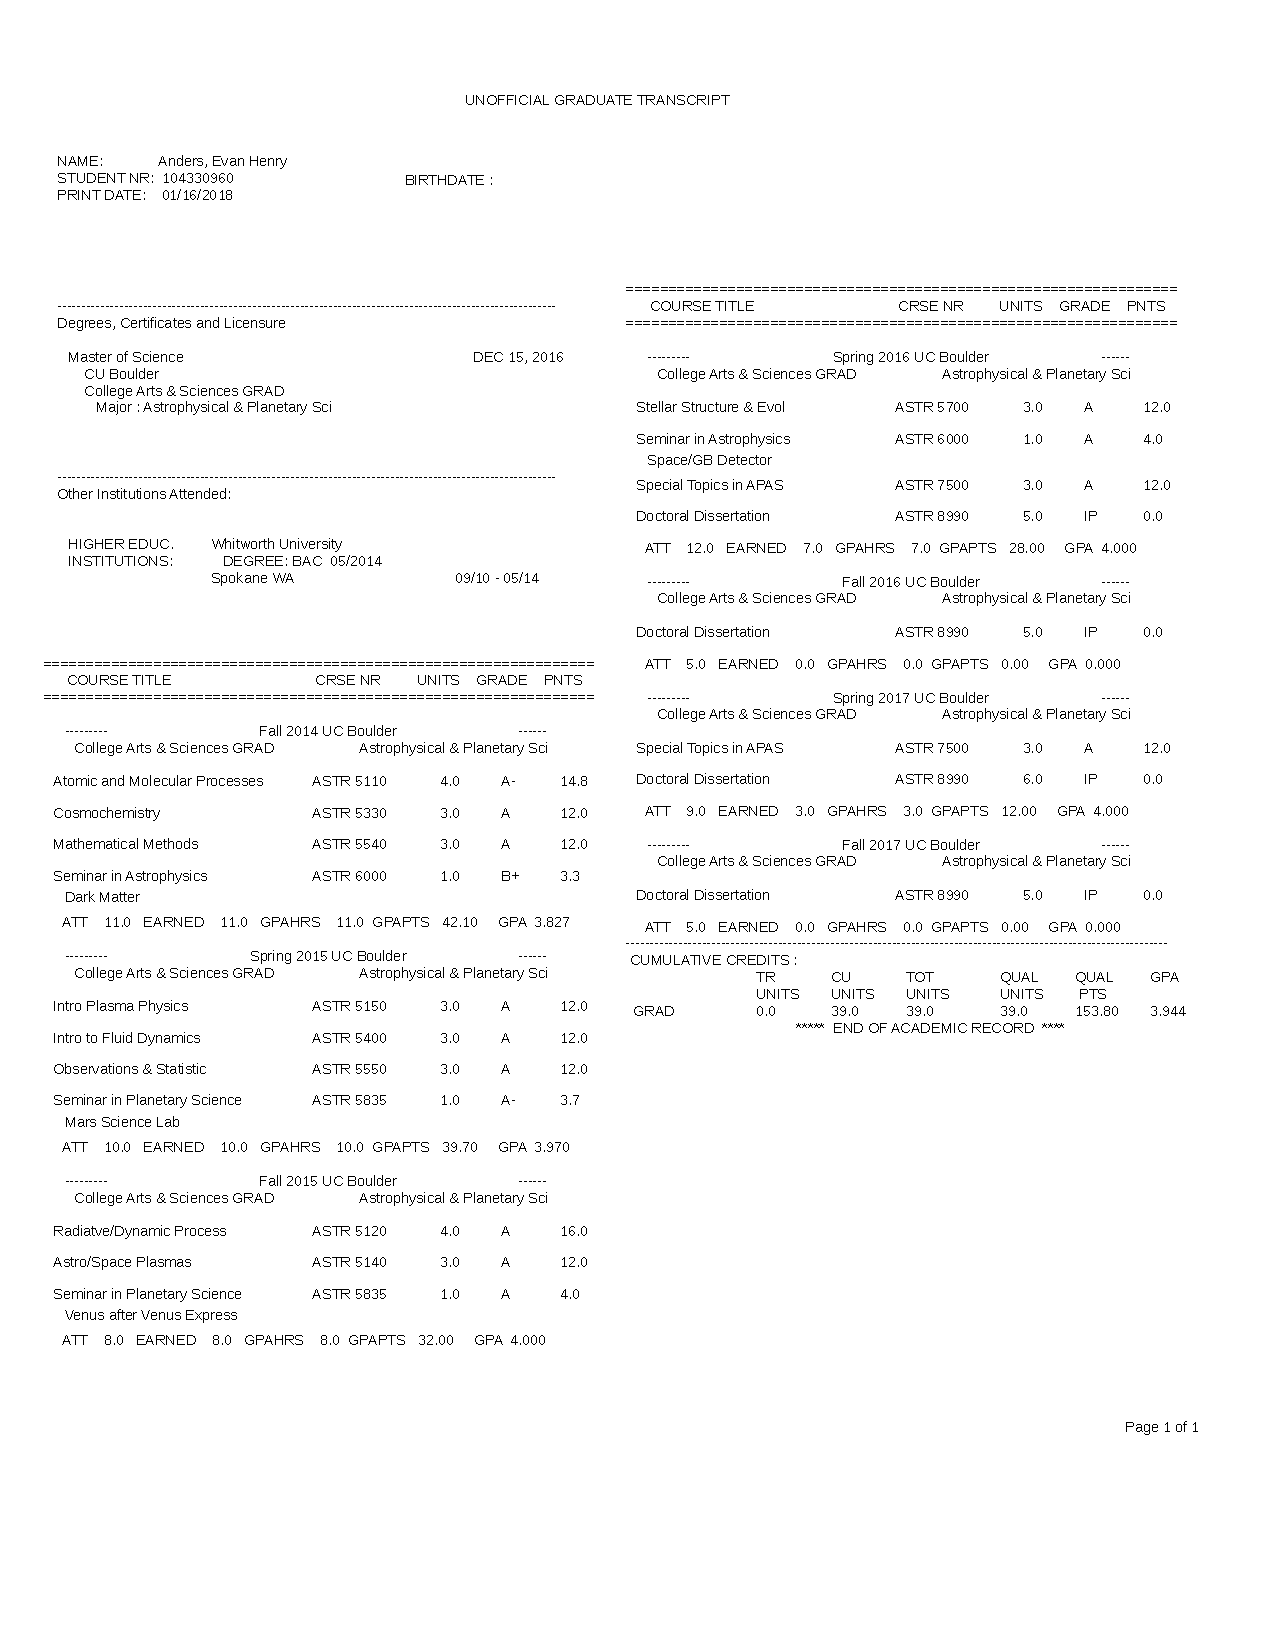
\includepdf[pages=-, pagecommand={}]{transcripts/transcript_cuFA2017_noPersonalInfo.pdf}


\bibliography{biblio}
\end{document}
